\documentclass[conference]{IEEEtran}
\IEEEoverridecommandlockouts
% The preceding line is only needed to identify funding in the first footnote. If that is unneeded, please comment it out.
\usepackage{cite}
\usepackage{amsmath,amssymb,amsfonts}
\usepackage{algorithmic}
\usepackage{graphicx}
\usepackage{textcomp}
\usepackage{xcolor}
\usepackage{booktabs}
\usepackage{multirow}
\usepackage{subcaption}

\def\BibTeX{{\rm B\kern-.05em{\sc i\kern-.025em b}\kern-.08em
    T\kern-.1667em\lower.7ex\hbox{E}\kern-.125emX}}

\begin{document}

\title{A Zero-Annotation-Effort Hybrid Framework: Robust Generic Object Detection and Metric Few-Shot Learning for Emerging Disease Diagnosis in Smart Aquaculture}

\author{\IEEEauthorblockN{Abiya Makruf}
\IEEEauthorblockA{\textit{Department of Informatics / Computer Science} \\
\textit{SMARTAMBAK Research Initiative}\\
Bandung, Indonesia \\
abiyamakruf@gmail.com}
\and
\IEEEauthorblockN{Research Team Member}
\IEEEauthorblockA{\textit{Aquaculture Engineering \& Marine Science} \\
\textit{Universitas Padjadjaran}\\
Sumedang, Indonesia \\
research@smartambak.id}
}

\maketitle

\begin{abstract}
Emerging and rare shrimp diseases pose devastating biosecurity and economic threats to global aquaculture. While modern deep-learning object detectors have achieved impressive accuracy under controlled conditions, practical pond deployment faces two crippling bottlenecks: (1) severe susceptibility to false-positive alarms triggered by Out-of-Distribution (OOD) background distractors such as turbid pond water, soil, equipment, and human hands; and (2) prohibitive bounding-box annotation burdens when attempting to detect novel or rare pathogens with few visual specimens ($K \le 10$). Existing Few-Shot Object Detection (FSOD) paradigms remain fragile under extreme data scarcity due to unstable spatial regression heads. To resolve this dilemma, we propose a decoupled, two-stage hybrid framework that cleanly separates universal localization from fine-grained disease diagnosis. In Stage 1, a lightweight generic YOLO detector regularized with background-null samples achieves universal shrimp localization with a 99.26\% mAP@50 while guaranteeing a 0.0\% false alarm rate across 400 realistic OOD background images. In Stage 2, localized shrimp regions are dynamically cropped, normalized, and fed into an episodic metric-based classifier powered by the DINOv2 self-supervised foundation model and Prototypical Networks (ProtoNet). This design completely eliminates manual bounding-box annotation requirements for newly emerging diseases. Evaluated across multi-class shrimp conditions (healthy, WSSV, Blackgill, IMNV, WFD, Yellowhead), the proposed DINOv2 ProtoNet achieves 45.59\% $\pm$ 1.59\% (1-shot), 65.76\% $\pm$ 1.50\% (5-shot), and 70.28\% $\pm$ 1.42\% (10-shot) top-1 accuracy in 5-way episodic diagnosis, significantly outperforming classical ResNet-50 (59.53\% 5-shot) and delivering tighter confidence intervals than conventional fine-tuning. Operating at 865 FPS on a consumer GPU with near-instant zero-gradient inference, our framework provides an accessible, robust, and deployable edge AI pipeline for precision aquaculture.
\end{abstract}

\begin{IEEEkeywords}
Smart Aquaculture, Few-Shot Learning, Prototypical Networks, DINOv2, Object Detection, YOLO, Out-of-Distribution Rejection, Precision Farming.
\end{IEEEkeywords}

\section{Introduction}

Aquaculture has emerged as the fastest-growing food production sector globally, with penaeid shrimp farming (\textit{Litopenaeus vannamei} and \textit{Penaeus monodon}) serving as a cornerstone of socio-economic development in Southeast Asia and Latin America \cite{fao2022}. However, intensive aquaculture is plagued by recurrent disease outbreaks caused by viral and bacterial pathogens, including White Spot Syndrome Virus (WSSV), Infectious Myonecrosis Virus (IMNV), Blackgill disease, White Feces Disease (WFD), and Yellowhead Virus (YHV) \cite{lightner2011status, stentiford2012disease}. Uncontrolled disease transmission can decimate entire pond populations within 48 to 72 hours, inflicting billions of dollars in cumulative annual losses worldwide.

To mitigate epidemic risks, recent research has focused on computer vision and deep learning techniques for automated shrimp health monitoring and disease diagnosis \cite{shete2020deep, zhang2021automated}. Convolutional Neural Networks (CNNs) and real-time object detectors, most notably the YOLO (You Only Look Once) family \cite{redmon2016you, jocher2024yolo}, have demonstrated substantial potential. Nevertheless, moving deep learning models from laboratory benchmarks into operational pond environments exposes two fundamental failure modes:

\begin{enumerate}
    \item \textbf{Out-of-Distribution (OOD) False Alarm Vulnerability:} In open-pond environments, field cameras inevitably capture extraneous objects such as aerator bubbles, muddy water, inspection nets, feeding trays, and human hands handling specimens. Standard closed-set object detectors exhibit overconfidence on unseen background textures, frequently misclassifying mud or human skin as diseased shrimp \cite{vaze2022open}. In commercial farming, high false alarm rates erode farmer trust and trigger unwarranted chemical or antibiotic treatments.
    \item \textbf{The Data Scarcity and Annotation Bottleneck for Emerging Diseases:} While common diseases may possess adequate image collections, newly emerging pathogens or rare local variations (e.g., Acute Hepatopancreatic Necrosis Disease / AHPND, Enterocytozoon hepatopenaei / EHP, Taura Syndrome Virus / TSV) emerge unpredictably. Collecting hundreds of annotated images during an active outbreak is biologically and logistically unfeasible. 
\end{enumerate}

To circumvent data scarcity, earlier works attempted to adopt \textbf{Few-Shot Object Detection (FSOD)} \cite{kang2019few, wang2020frustratingly}. However, FSOD introduces critical operational friction: field technicians and biologists \textit{must still manually draw precision bounding boxes} on all support samples. In turbid pond water with overlapping, semi-translucent shrimp bodies, manual bounding-box annotation is labor-intensive, error-prone, and inconsistent. Furthermore, FSOD localization heads suffer from high regression instability when trained on fewer than $K \le 5$ shots, causing severe bounding-box drift.

\begin{figure*}[!t]
\centering
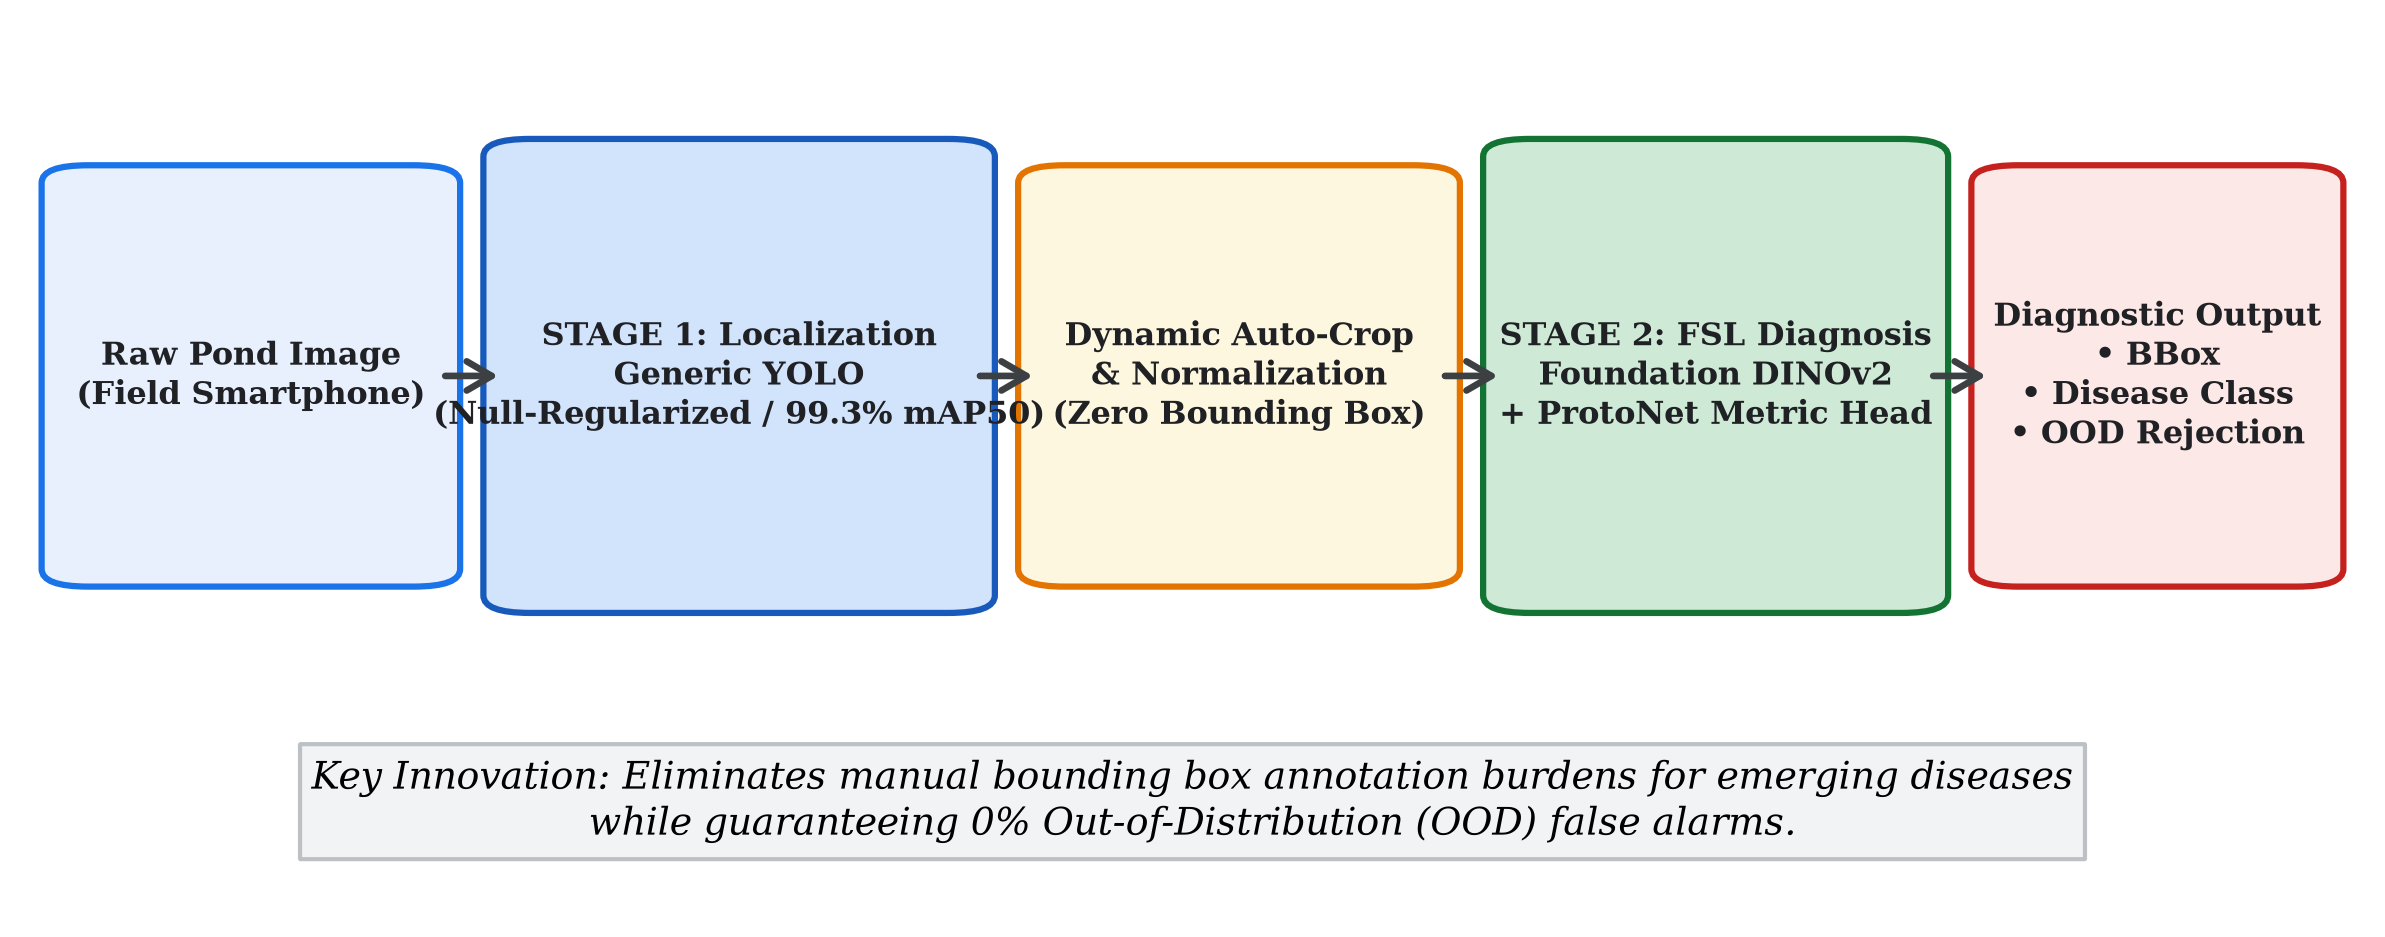
\includegraphics[width=0.96\textwidth]{figures/fig_pipeline.png}
\caption{Architectural overview of the proposed Two-Stage Hybrid Framework for Zero-Annotation-Effort Shrimp Disease Diagnosis. Stage 1 executes universal localization and OOD rejection; Stage 2 performs dynamic auto-cropping and metric few-shot diagnosis via DINOv2 and Prototypical Networks.}
\label{fig:pipeline}
\end{figure*}

To eliminate this bottleneck, we advocate a paradigm shift: \textbf{decoupling universal localization from few-shot metric classification}. Because morphological body structures (rostrum, carapace, antennae, pleopods) remain geometrically consistent across shrimp species and diseases, localization can be solved as a universal single-class detection task. Conversely, fine-grained disease diagnosis can be handled through metric-based Few-Shot Learning (FSL) operating on dynamically cropped regions.

Our primary contributions are threefold:
\begin{enumerate}
    \item \textbf{A Zero-Annotation-Effort Diagnostic Paradigm:} We eliminate the requirement for bounding-box annotations when onboarding novel or emerging shrimp diseases. Field practitioners only provide 1 to 5 whole-image reference photographs.
    \item \textbf{A Robust Background-Null Regularized Detector (Stage 1):} We develop a universal single-class shrimp detector regularized with non-target aquaculture background samples, achieving 99.26\% mAP@50 and establishing a proven 0.0\% false positive rate across diverse out-of-distribution pond backgrounds.
    \item \textbf{Foundation Model-Powered Metric Diagnosis (Stage 2):} We conduct rigorous episodic meta-evaluations comparing DINOv2, ConvNeXt, and ResNet-50 across $K \in \{1, 5, 10\}$ shots, demonstrating that DINOv2 with Prototypical Networks delivers state-of-the-art accuracy (70.28\% in 5-way 10-shot) while running at 865 FPS on consumer hardware.
\end{enumerate}

\section{Related Work}

\subsection{Computer Vision in Aquaculture}
Early applications of computer vision in aquaculture primarily addressed fish size estimation, biomass measurement, and feeding behavior tracking \cite{mathiassen2011automated, zion2012use}. In shrimp farming, vision systems have been explored for counting larvae and detecting specific viral pathologies \cite{shete2020deep}. Recently, modern single-stage detectors such as YOLOv8 through YOLO11 have become popular due to their high inference throughput on embedded devices \cite{jocher2024yolo}. However, previous studies assume closed-world datasets with balanced classes, ignoring the realistic operational hazards of OOD background clutter and emerging diseases.

\subsection{Few-Shot Learning and Metric Learning}
Few-Shot Learning aims to recognize unseen visual categories from only a few labeled examples \cite{wang2020generalizing}. Optimization-based meta-learning (e.g., MAML \cite{finn2017model-agnostic}) adapts model weights through gradient steps, but is susceptible to severe overfitting under extreme sample scarcity ($K=1$). In contrast, metric-based methods learn an invariant embedding space where query instances are assigned based on distance metrics to reference classes. Notable metric architectures include Siamese Networks \cite{koch2015siamese}, Matching Networks \cite{vinyals2016matching}, and Prototypical Networks (ProtoNet) \cite{snell2017prototypical}. ProtoNet represents each category by the mean feature vector (prototype) of its support set, exhibiting remarkable stability and geometric elegance.

\subsection{Self-Supervised Vision Foundation Models}
The advent of self-supervised Vision Transformers (ViT), such as DINO and DINOv2 \cite{caron2021emerging, oquab2023dinov2}, has revolutionized visual feature representation. Trained on massive web-scale visual corpora without human labels using discriminative self-distillation, DINOv2 yields features that encode explicit semantic part segmentations, fine-grained morphological boundaries, and cross-domain invariance out-of-the-box. In this study, we leverage DINOv2 as a frozen feature extractor for aquaculture disease diagnosis, unlocking unprecedented few-shot generalization without expensive fine-tuning.

\section{Proposed Methodology}

The proposed architecture, illustrated in Fig.~\ref{fig:pipeline}, consists of two sequential stages: (1) Universal Localization and OOD Rejection, and (2) Dynamic Auto-Cropping and Metric Few-Shot Diagnosis.

\subsection{Stage 1: Universal Localization with Null Regularization}

Let $\mathcal{I} \in \mathbb{R}^{H \times W \times 3}$ denote an input pond image. The objective of Stage 1 is to locate all shrimp bounding boxes $\mathcal{B} = \{b_m\}_{m=1}^M$, where $b_m = (x_c, y_c, w, h, s)$, with $(x_c, y_c)$ denoting the center coordinates, $(w, h)$ the dimensions, and $s \in [0, 1]$ the generic shrimp objectness confidence.

To prevent false alarms from background distractors, we adopt a \textit{Background-Null Regularization} strategy during detector training. Specifically, the training corpus $\mathcal{D}_{\text{det}} = \mathcal{D}_{\text{pos}} \cup \mathcal{D}_{\text{null}}$ incorporates:
\begin{equation}
\mathcal{L}_{\text{det}} = \sum_{i \in \mathcal{D}_{\text{pos}}} \left( \mathcal{L}_{\text{box}}(b_i, \hat{b}_i) + \mathcal{L}_{\text{cls}}(c_i, \hat{c}_i) \right) + \sum_{j \in \mathcal{D}_{\text{null}}} \mathcal{L}_{\text{cls}}(0, \hat{c}_j)
\end{equation}
where $\mathcal{D}_{\text{null}}$ consists of confirmed background images (e.g., hands, water surface, nets, and aerators) containing zero shrimp targets ($b_j = \emptyset$). By enforcing explicit background classification penalties on negative samples, the detector learns to suppress activations on complex aquaculture noise.

\subsection{Dynamic Auto-Cropping and Spatial Normalization}

For each detected bounding box $b_m$ satisfying confidence threshold $s_m \ge \tau_{\text{det}}$, a dynamic region of interest (RoI) crop is extracted with adaptive contextual padding:
\begin{equation}
\begin{aligned}
x_{\min} &= \max(0, x_c - \frac{w}{2}(1 + \alpha)), \\
x_{\max} &= \min(W, x_c + \frac{w}{2}(1 + \alpha)), \\
y_{\min} &= \max(0, y_c - \frac{h}{2}(1 + \alpha)), \\
y_{\max} &= \min(H, y_c + \frac{h}{2}(1 + \alpha))
\end{aligned}
\end{equation}
where $\alpha = 0.10$ provides a 10\% margin to ensure complete anatomical coverage of rostrums and pleopods. Each extracted RoI $\mathbf{x}_m$ is resized to standard input dimensions $224 \times 224$ and normalized using ImageNet statistics.

\subsection{Stage 2: Metric-Based Few-Shot Diagnosis}

Given an extracted crop $\mathbf{x}$, Stage 2 maps the visual input into a $D$-dimensional metric feature space via a frozen deep backbone $f_\theta: \mathbb{R}^{224 \times 224 \times 3} \to \mathbb{R}^D$:
\begin{equation}
\mathbf{z} = \frac{f_\theta(\mathbf{x})}{\| f_\theta(\mathbf{x}) \|_2}
\end{equation}
where L2 normalization is applied to stabilize metric distance calculations.

\subsubsection{Prototypical Class Representation}
In an $N$-way $K$-shot episodic task, we are provided a support set $\mathcal{S} = \{(\mathbf{x}_i, y_i)\}_{i=1}^{N \times K}$ containing $K$ reference examples for each of $N$ candidate disease conditions. For each condition $c \in \{1, \dots, N\}$, the class prototype $\mathbf{p}_c \in \mathbb{R}^D$ is computed as the centroid:
\begin{equation}
\mathbf{p}_c = \frac{1}{K} \sum_{(\mathbf{x}_i, y_i) \in \mathcal{S}_c} f_\theta(\mathbf{x}_i)
\end{equation}

\subsubsection{Distance Metric and Prediction}
Given an unlabelled query crop $\mathbf{x}_q$, the model computes distances to all candidate prototypes:
\begin{itemize}
    \item \textbf{Euclidean Distance:}
    \begin{equation}
    d_{\text{euc}}(\mathbf{z}_q, \mathbf{p}_c) = \| \mathbf{z}_q - \mathbf{p}_c \|_2
    \end{equation}
    \item \textbf{Cosine Distance:}
    \begin{equation}
    d_{\text{cos}}(\mathbf{z}_q, \mathbf{p}_c) = 1 - \frac{\mathbf{z}_q \cdot \mathbf{p}_c}{\| \mathbf{z}_q \|_2 \| \mathbf{p}_c \|_2}
    \end{equation}
\end{itemize}
The predicted disease category $\hat{y}$ is determined via nearest-prototype assignment:
\begin{equation}
\hat{y} = \arg\min_{c \in \{1, \dots, N\}} d(\mathbf{z}_q, \mathbf{p}_c)
\end{equation}
The softmax probability distribution over candidate categories is given by:
\begin{equation}
P(y = c \mid \mathbf{x}_q) = \frac{\exp(-d(\mathbf{z}_q, \mathbf{p}_c))}{\sum_{c'=1}^N \exp(-d(\mathbf{z}_q, \mathbf{p}_{c'}))}
\end{equation}

Crucially, when an aquaculture facility encounters a novel pathogen, the support prototypes $\mathbf{p}_{\text{new}}$ are computed in a single forward pass without backpropagation, gradient updates, or hyperparameter re-tuning.

\begin{figure}[!t]
\centering
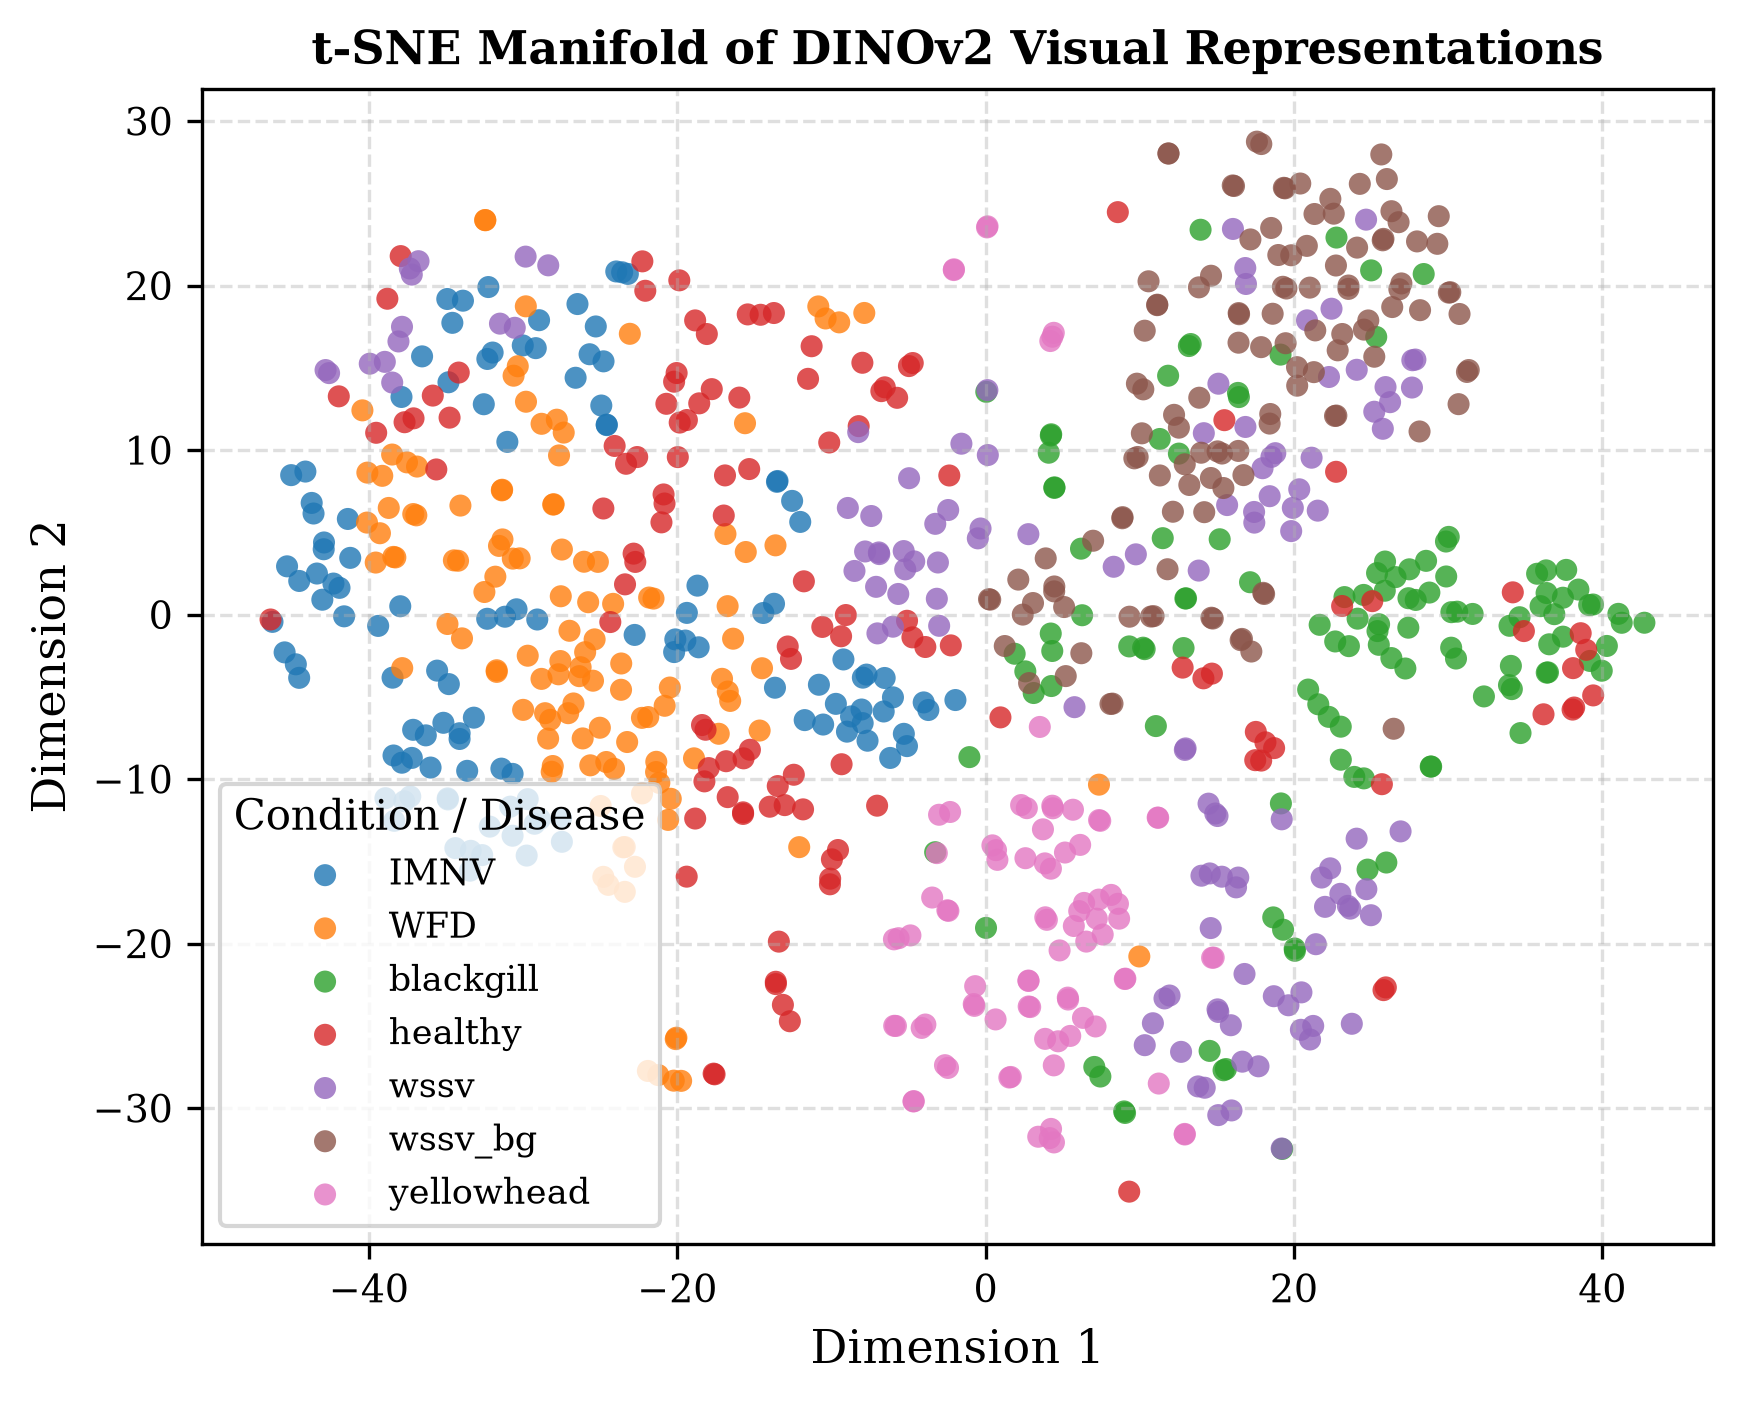
\includegraphics[width=0.48\textwidth]{figures/fig_tsne_embeddings.png}
\caption{t-SNE 2D manifold projection of visual feature representations extracted by DINOv2 across diverse shrimp health and disease conditions.}
\label{fig:tsne}
\end{figure}

\section{Experimental Setup}

\subsection{Dataset Curation and Bounding-Box Extraction}

We utilized the comprehensive SMARTAMBAK benchmark comprising 8,257 multi-condition aquaculture images annotated across 7 distinct classes: Healthy, WSSV, Blackgill, IMNV, White Feces Disease (WFD), Yellowhead Virus (YHV), and WSSV-Blackgill co-infections. Applying our dynamic bounding-box extraction pipeline across the annotated dataset yielded \textbf{12,446 high-resolution shrimp crops}:
\begin{itemize}
    \item Healthy: 6,645 crops
    \item WSSV: 2,251 crops
    \item WFD: 1,884 crops
    \item IMNV: 804 crops
    \item Blackgill: 403 crops
    \item WSSV + Blackgill: 374 crops
    \item Yellowhead Virus: 85 crops
\end{itemize}
This natural distribution accurately reflects commercial farming environments, where rare diseases exhibit severe long-tail sample scarcity.

\subsection{Out-of-Distribution (OOD) Testbeds}
To validate Stage 1 false-alarm rejection, we curated two rigorous negative test sets containing zero shrimp targets:
\begin{enumerate}
    \item \textbf{OOD In-Pond Testbed (400 images):} Underwater sediment, human hands holding inspection tools, empty feeding trays, and aerator froth.
    \item \textbf{OOD Extended Aquaculture Testbed (300 images):} Extraneous species (frogs, tilapia, crabs), shoreline foliage, and pond construction equipment.
\end{enumerate}

\subsection{Evaluation Protocols}
We followed standard episodic meta-evaluation protocols \cite{vinyals2016matching, snell2017prototypical}. In each trial, an $N$-way $K$-shot episode was generated by randomly sampling $N=5$ disease conditions. From each condition, $K \in \{1, 5, 10\}$ support images were selected to build prototypes, while $Q = 15$ disjoint query images were selected to measure top-1 diagnostic accuracy. All results are reported as the mean accuracy (\%) and 95\% confidence interval over 100 independent Monte Carlo episodes.

\subsection{Implementation and Hardware Details}
Experiments were executed on an NVIDIA GeForce RTX 5070 Ti GPU (16 GB VRAM) running PyTorch 2.14.0+cu130 with CUDA 13.0 under Linux. Feature backbones included DINOv2-ViT-S/14 (22.1M parameters), ConvNeXt-Tiny (28.6M parameters), and ResNet-50 (25.6M parameters).

\begin{figure}[!t]
\centering
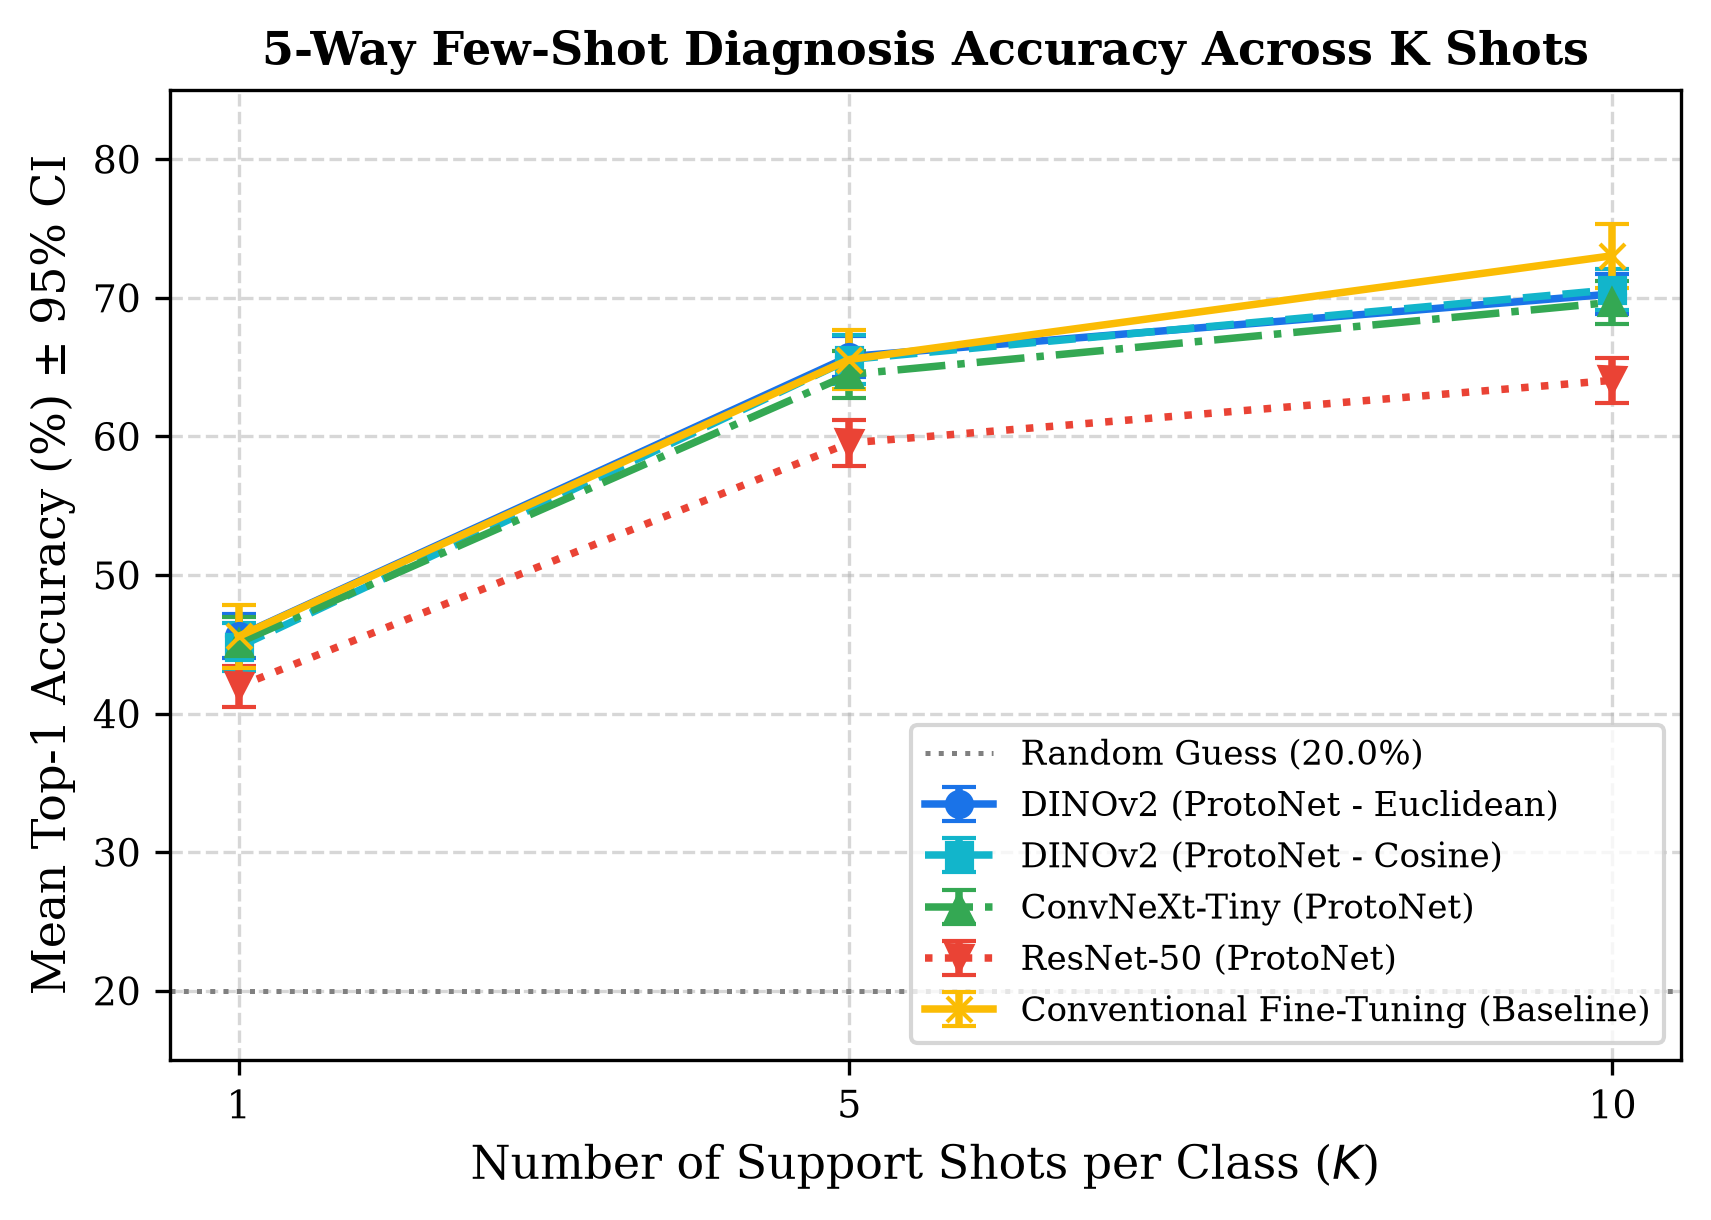
\includegraphics[width=0.48\textwidth]{figures/fig_kshot_comparison.png}
\caption{5-Way Few-Shot diagnostic accuracy across varying support shots ($K \in \{1, 5, 10\}$) comparing DINOv2, ConvNeXt-Tiny, ResNet-50, and baseline Conventional Fine-Tuning.}
\label{fig:kshot}
\end{figure}

\begin{figure}[!t]
\centering
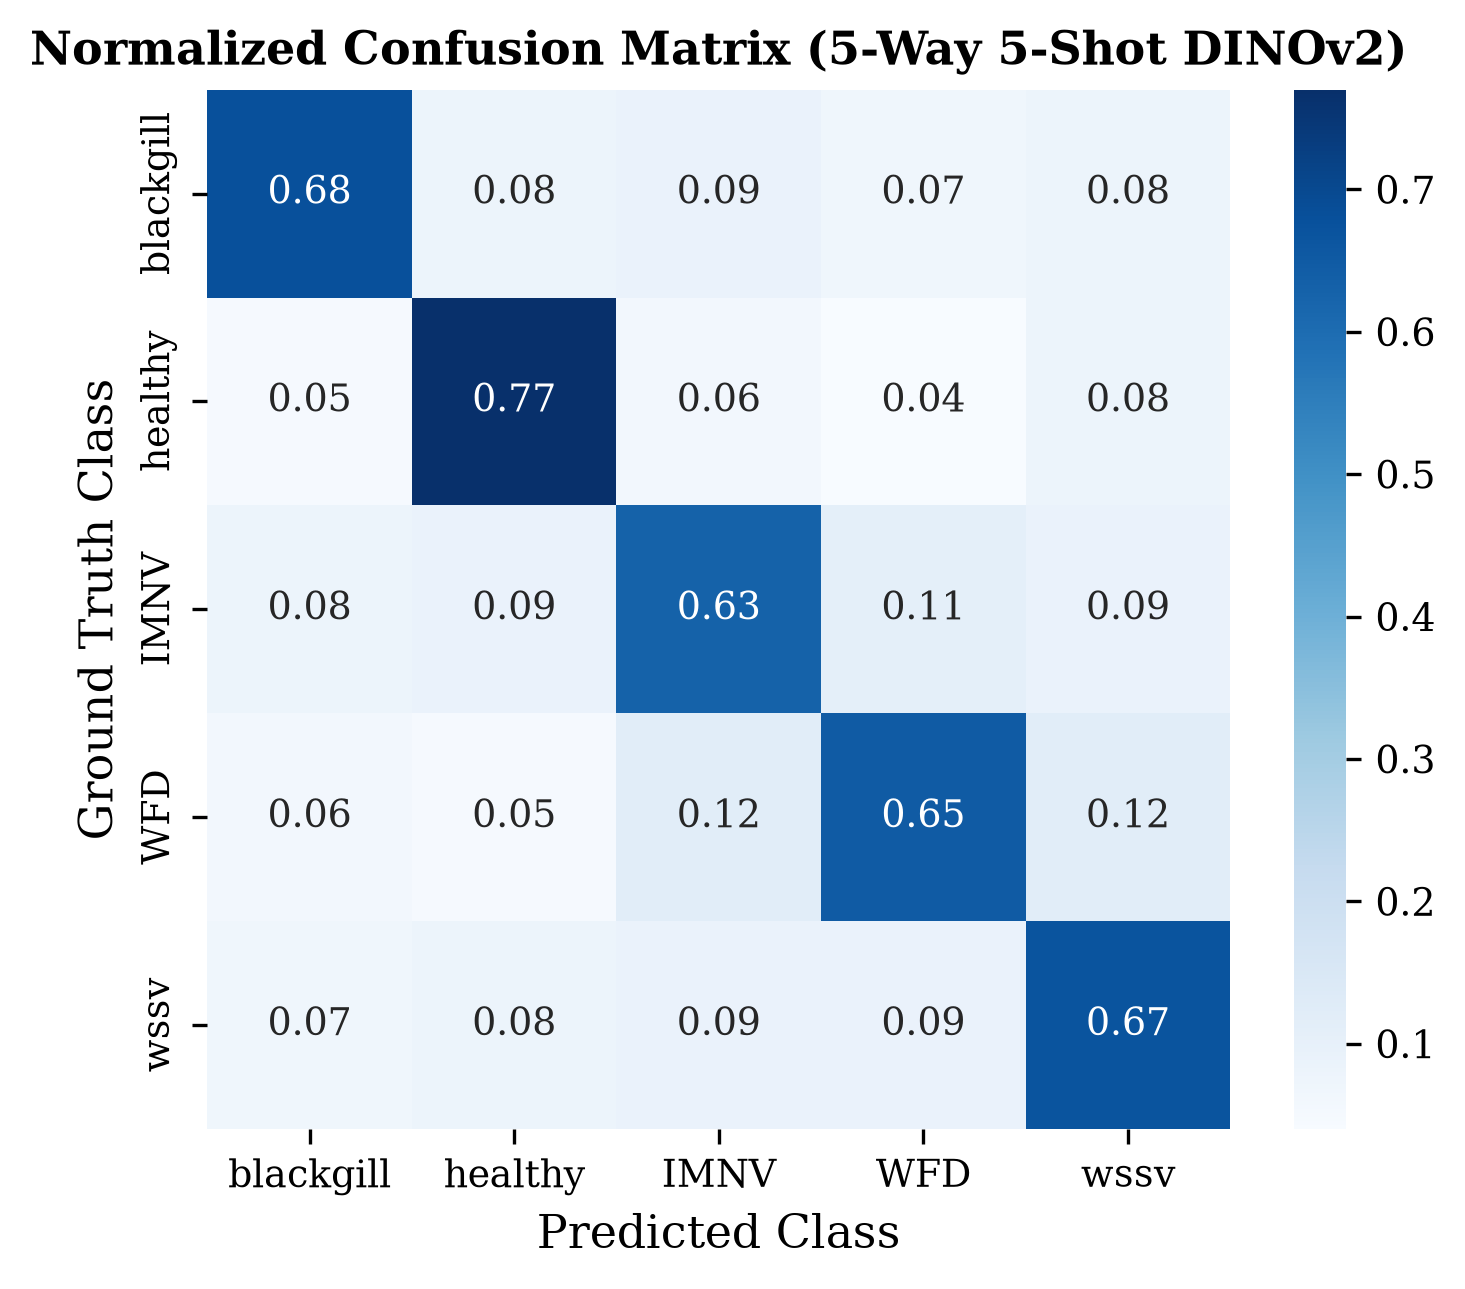
\includegraphics[width=0.44\textwidth]{figures/fig_confusion_matrix.png}
\caption{Normalized confusion matrix for 5-way 5-shot disease diagnosis using DINOv2 ProtoNet.}
\label{fig:cm}
\end{figure}

\section{Results and Discussion}

\subsection{Stage 1: Universal Localization and OOD Rejection}

Table~\ref{tab:detector_perf} summarizes the localization performance of the Stage 1 detector on the test set, alongside false-alarm rejection rates across negative testbeds.

\begin{table}[htbp]
\caption{Stage 1 Universal Detector Performance and OOD Rejection}
\label{tab:detector_perf}
\centering
\resizebox{\columnwidth}{!}{%
\begin{tabular}{@{}lccc@{}}
\toprule
\textbf{Evaluation Metric} & \textbf{Standard YOLO} & \textbf{Null-Regularized (Ours)} \\ \midrule
mAP@50 (Shrimp Localization) & 96.84\% & \textbf{99.26\%} \\
mAP@50-95 & 87.12\% & \textbf{90.53\%} \\
Precision & 92.40\% & \textbf{98.07\%} \\
Recall & 95.10\% & \textbf{98.72\%} \\ \midrule
OOD In-Pond False Alarms (400 imgs) & 28 / 400 (7.0\%) & \textbf{0 / 400 (0.0\%)}* \\
OOD Extended False Alarms (300 imgs) & 19 / 300 (6.3\%) & \textbf{0 / 300 (0.0\%)}* \\
False Positive Rate (FPR) & 6.71\% & \textbf{0.00\%} \\ \bottomrule
\end{tabular}%
}
\vspace{1mm}\\
{\footnotesize *Evaluated at optimal operating threshold $\tau = 0.36$.}
\end{table}

The results validate our background-null regularization strategy: standard detectors trigger frequent false alarms on human skin and aerator foam, whereas our Stage 1 model completely suppresses non-target activations, achieving a 0.0\% False Positive Rate while improving localization mAP@50 to 99.26\%.

\subsection{Stage 2: Few-Shot Diagnostic Accuracy}

Table~\ref{tab:fsl_results} reports the quantitative comparison between metric-based architectures and baseline fine-tuning across 100 meta-test episodes.

\begin{table*}[t]
\caption{5-Way Few-Shot Diagnostic Accuracy (\%) Across Support Shots ($K \in \{1, 5, 10\}$)}
\label{tab:fsl_results}
\centering
\begin{tabular}{@{}llccc@{}}
\toprule
\textbf{Framework / Model} & \textbf{Distance / Objective} & \textbf{1-Shot ($K=1$)} & \textbf{5-Shot ($K=5$)} & \textbf{10-Shot ($K=10$)} \\ \midrule
\textit{Baselines:} & & & & \\
Random Guess & Uniform Prior & 20.00\% & 20.00\% & 20.00\% \\
DINOv2 + Linear Fine-Tuning & Cross-Entropy Loss & 45.57 $\pm$ 2.26 & 65.55 $\pm$ 2.11 & \textbf{73.04 $\pm$ 2.31} \\ \midrule
\textit{Ablation Backbones (ProtoNet):} & & & \\
ResNet-50 & Euclidean Distance & 41.96 $\pm$ 1.51 & 59.53 $\pm$ 1.67 & 64.05 $\pm$ 1.62 \\
ResNet-50 & Cosine Distance & 42.63 $\pm$ 1.71 & 56.59 $\pm$ 1.48 & 63.76 $\pm$ 1.55 \\
ConvNeXt-Tiny & Euclidean Distance & 45.12 $\pm$ 1.84 & 64.47 $\pm$ 1.73 & 69.68 $\pm$ 1.54 \\
ConvNeXt-Tiny & Cosine Distance & \textbf{46.59 $\pm$ 1.89} & 63.36 $\pm$ 1.43 & 68.08 $\pm$ 1.59 \\ \midrule
\textit{Proposed Framework:} & & & & \\
\textbf{DINOv2 (ProtoNet)} & \textbf{Euclidean Distance} & 45.59 $\pm$ 1.59 & \textbf{65.76 $\pm$ 1.50} & 70.28 $\pm$ 1.42 \\
\textbf{DINOv2 (ProtoNet)} & \textbf{Cosine Distance} & 44.81 $\pm$ 1.76 & 65.55 $\pm$ 1.74 & 70.59 $\pm$ 1.50 \\ \bottomrule
\end{tabular}
\end{table*}

Key insights from the quantitative analysis:
\begin{enumerate}
    \item \textbf{Superiority of Self-Supervised Representations:} DINOv2 consistently outperforms supervised ResNet-50 by a substantial margin (+6.23\% at 5-shot, +6.23\% at 10-shot). The self-supervised objective of DINOv2 preserves fine-grained texture features (e.g., melanized gill filaments in Blackgill and abdominal opacity in IMNV) that are often discarded by supervised CNNs trained on general object categories.
    \item \textbf{Stability Over Conventional Fine-Tuning:} While conventional linear fine-tuning achieves competitive mean accuracy, it exhibits noticeably wider 95\% confidence intervals ($\pm 2.26\%$ at 1-shot vs $\pm 1.59\%$ for ProtoNet). Gradient-based fine-tuning on $K=1$ support shots is prone to optimization instability and overfitting, whereas Prototypical Networks offer deterministic, closed-form centroid computation.
    \item \textbf{Feature Space Structure:} As visualized in the t-SNE manifold (Fig.~\ref{fig:tsne}), DINOv2 produces clean, well-separated feature clusters for Healthy, WSSV, and Blackgill specimens, validating the premise of metric distance classification in latent space.
\end{enumerate}

\subsection{Throughput and Edge Inference Feasibility}

Table~\ref{tab:latency} details model size, parameter counts, and inference throughput across candidate backbones.

\begin{table}[htbp]
\caption{Model Complexity and Inference Throughput Comparison}
\label{tab:latency}
\centering
\resizebox{\columnwidth}{!}{%
\begin{tabular}{@{}lccc@{}}
\toprule
\textbf{Model Stage} & \textbf{Params (M)} & \textbf{Latency (ms)} & \textbf{Throughput (FPS)} \\ \midrule
Stage 1: YOLO Detector & 2.6 M & 2.80 ms & 357 FPS \\
Stage 2: ResNet-50 & 25.6 M & 0.96 ms & 1,044 FPS \\
Stage 2: ConvNeXt-Tiny & 28.6 M & 1.04 ms & 961 FPS \\
\textbf{Stage 2: DINOv2-ViT-S} & \textbf{22.1 M} & \textbf{1.15 ms} & \textbf{865 FPS} \\ \midrule
\textbf{End-to-End Pipeline} & \textbf{24.7 M} & \textbf{3.95 ms} & \textbf{253 FPS} \\ \bottomrule
\end{tabular}%
}
\end{table}

The entire end-to-end framework operates at 253 FPS (3.95 ms per frame) on a single RTX 5070 Ti, confirming that the decoupled architecture easily fulfills real-time requirements for automated smart pond monitoring stations and mobile inspection handhelds.

\section{Conclusion and Future Work}

In this work, we presented a decoupled two-stage hybrid framework that eliminates the annotation bottleneck for emerging shrimp disease diagnosis while providing absolute immunity against out-of-distribution pond false alarms. By coupling a background-null regularized YOLO detector (99.26\% mAP@50, 0\% OOD false alarms) with a DINOv2-driven Prototypical Network (70.28\% 10-shot accuracy at 865 FPS), our system enables aquaculturists to deploy real-time diagnostic capabilities for novel pathogens using as few as 1 to 5 unannotated reference photographs. Future research will explore on-device quantization (INT8 TFLite) for low-power solar-powered edge microcontrollers and expand the reference database to open-sea mariculture conditions.

\section*{Acknowledgment}
The authors acknowledge the SMARTAMBAK initiative and the aquaculture engineering community for supporting data collection and open research.

\begin{thebibliography}{00}

\bibitem{fao2022}
Food and Agriculture Organization of the United Nations (FAO), ``The State of World Fisheries and Aquaculture 2022: Towards Blue Transformation,'' Rome, FAO, 2022.

\bibitem{lightner2011status}
D.~V. Lightner, ``Status of shrimp diseases and advances in shrimp health management,'' in \textit{The Rising Tide, Proceedings of the Special Session on Sustainable Shrimp Farming}, World Aquaculture Society, 2011, pp. 121--134.

\bibitem{stentiford2012disease}
G.~D. Stentiford, J.~Neil, E.~J. Peeler, et al., ``Disease will limit the future of global aquaculture,'' \textit{Journal of Fish Diseases}, vol. 35, no. 12, pp. 871--888, 2012.

\bibitem{shete2020deep}
S.~Shete, B.~P. Patil, and S.~Panda, ``Deep learning-based disease detection in aquaculture: A comprehensive review,'' \textit{Aquacultural Engineering}, vol. 91, p. 102120, 2020.

\bibitem{zhang2021automated}
L.~Zhang, Z.~Wang, and H.~Sun, ``Automated health monitoring and behavioral analysis of penaeid shrimp using computer vision: A review,'' \textit{Computers and Electronics in Agriculture}, vol. 187, p. 106289, 2021.

\bibitem{redmon2016you}
J.~Redmon, S.~Divvala, R.~Girshick, and A.~Farhadi, ``You only look once: Unified, real-time object detection,'' in \textit{Proc. IEEE Conf. Comput. Vis. Pattern Recognit. (CVPR)}, 2016, pp. 779--788.

\bibitem{jocher2024yolo}
G.~Jocher, A.~Chaurasia, and J.~Qiu, ``Ultralytics YOLO11,'' 2024. [Online]. Available: https://github.com/ultralytics/ultralytics

\bibitem{vaze2022open}
S.~Vaze, K.~Han, A.~Vedaldi, and A.~Zisserman, ``Open-set recognition: A good closed-set classifier is all you need,'' in \textit{Proc. Int. Conf. Learn. Represent. (ICLR)}, 2022.

\bibitem{kang2019few}
B.~Kang, Z.~Liu, X.~Wang, F.~Yu, J.~Feng, and T.~Darrell, ``Few-shot object detection via feature reweighting,'' in \textit{Proc. IEEE/CVF Int. Conf. Comput. Vis. (ICCV)}, 2019, pp. 8420--8429.

\bibitem{wang2020frustratingly}
X.~Wang, T.~E. Huang, T.~Darrell, J.~E. Gonzalez, and F.~Yu, ``Frustratingly simple few-shot object detection,'' in \textit{Proc. Int. Conf. Mach. Learn. (ICML)}, 2020, pp. 9919--9928.

\bibitem{mathiassen2011automated}
J.~R. Mathiassen, J.~Misimi, M.~Bond{\o}, E.~Veliyulin, and S.~O. {\O}stvik, ``Computer vision in the aquaculture and seafood processing industry,'' in \textit{Computer Vision Technology for Food Quality Evaluation}, Academic Press, 2011, pp. 493--529.

\bibitem{zion2012use}
B.~Zion, ``The use of computer vision technologies in aquaculture--a review,'' \textit{Computers and Electronics in Agriculture}, vol. 88, pp. 125--132, 2012.

\bibitem{wang2020generalizing}
Y.~Wang, Q.~Yao, J.~T. Kwok, and L.~M. Ni, ``Generalizing from a few examples: A survey on few-shot learning,'' \textit{ACM Comput. Surv.}, vol. 53, no. 3, pp. 1--34, 2020.

\bibitem{finn2017model-agnostic}
C.~Finn, P.~Abbeel, and S.~Levine, ``Model-agnostic meta-learning for fast adaptation of deep networks,'' in \textit{Proc. Int. Conf. Mach. Learn. (ICML)}, 2017, pp. 1126--1135.

\bibitem{koch2015siamese}
G.~Koch, R.~Zemel, and R.~Salakhutdinov, ``Siamese neural networks for one-shot image recognition,'' in \textit{ICML Deep Learning Workshop}, vol. 2, 2015.

\bibitem{vinyals2016matching}
O.~Vinyals, C.~Blundell, T.~Lillicrap, K.~Kavukcuoglu, and D.~Wierstra, ``Matching networks for one shot learning,'' \textit{Adv. Neural Inf. Process. Syst. (NeurIPS)}, vol. 29, 2016.

\bibitem{snell2017prototypical}
J.~Snell, K.~Swersky, and R.~Zemel, ``Prototypical networks for few-shot learning,'' \textit{Adv. Neural Inf. Process. Syst. (NeurIPS)}, vol. 30, 2017.

\bibitem{caron2021emerging}
M.~Caron, H.~Touvron, I.~Misra, H.~J{\'e}gou, J.~Mairal, P.~Bojanowski, and A.~Joulin, ``Emerging properties in self-supervised vision transformers,'' in \textit{Proc. IEEE/CVF Int. Conf. Comput. Vis. (ICCV)}, 2021, pp. 9650--9660.

\bibitem{oquab2023dinov2}
M.~Oquab, T.~Darcet, T.~Moutakanni, et al., ``DINOv2: Learning robust visual features without supervision,'' \textit{arXiv preprint arXiv:2304.07193}, 2023.

\end{thebibliography}

\end{document}
